% Created 2020-07-09 jeu. 15:28
% Intended LaTeX compiler: pdflatex
\documentclass{elsarticle}
\usepackage[utf8]{inputenc}
\usepackage[T1]{fontenc}
\usepackage{graphicx}
\usepackage{grffile}
\usepackage{longtable}
\usepackage{wrapfig}
\usepackage{rotating}
\usepackage[normalem]{ulem}
\usepackage{amsmath}
\usepackage{textcomp}
\usepackage{amssymb}
\usepackage{capt-of}
\usepackage{hyperref}
\usepackage{color}
\usepackage{minted}             % pour de jolis blocs de code
\usepackage{lineno,hyperref}
\modulolinenumbers[5]
\journal{Journal of \LaTeX\ Templates}
\bibliographystyle{model5-names}\biboptions{authoryear}
\date{\today}
\title{}
\hypersetup{
 pdfauthor={Frédéric Santos},
 pdftitle={},
 pdfkeywords={},
 pdfsubject={},
 pdfcreator={Emacs 26.3 (Org mode 9.3.7)}, 
 pdflang={English}}
\begin{document}


\begin{frontmatter}

\title{DSP2 method}
\tnotetext[mytitlenote]{Fully documented templates are available in the elsarticle package on \href{http://www.ctan.org/tex-archive/macros/latex/contrib/elsarticle}{CTAN}.}

%% Group authors per affiliation:
\author{Elsevier\fnref{myfootnote}}
\address{Radarweg 29, Amsterdam}
\fntext[myfootnote]{Since 1880.}

%% or include affiliations in footnotes:
\author[mymainaddress,mysecondaryaddress]{Elsevier Inc}
\ead[url]{www.elsevier.com}

\author[mysecondaryaddress]{Global Customer Service\corref{mycorrespondingauthor}}
\cortext[mycorrespondingauthor]{Corresponding author}
\ead{support@elsevier.com}

\address[mymainaddress]{1600 John F Kennedy Boulevard, Philadelphia}
\address[mysecondaryaddress]{360 Park Avenue South, New York}

\begin{abstract}
This template helps you to create a properly formatted \LaTeX\ manuscript.
\end{abstract}

\begin{keyword}
\texttt{elsarticle.cls}\sep \LaTeX\sep Elsevier \sep template
\MSC[2010] 00-01\sep  99-00
\end{keyword}

\end{frontmatter}

\linenumbers
\section{Introduction}
\label{sec:org7934d55}
Lorem ipsum dolor sit amet, consectetuer adipiscing elit.  Donec hendrerit tempor tellus.  Donec pretium posuere tellus.  Proin quam nisl, tincidunt et, mattis eget, convallis nec, purus.  Cum sociis natoque penatibus et magnis dis parturient montes, nascetur ridiculus mus.  Nulla posuere.  Donec vitae dolor.  Nullam tristique diam non turpis.  Cras placerat accumsan nulla.  Nullam rutrum.  Nam vestibulum accumsan nisl.

\section{Material and methods}
\label{sec:orgc81ddec}
\subsection{Sample}
\label{sec:org1d96131}
The reference sample used in this study has been collected by \cite{bruzek2002_MethodVisualDetermination}. It is described in Table \ref{tab-sample}.

\begin{table}[htbp]
\centering
\begin{tabular}{lrr}
 & F & M\\
\hline
Geneva & 64 & 70\\
Maxwell & 49 & 58\\
\end{tabular}
\caption{Description of the reference sample. \label{tab-sample}}

\end{table}

\subsection{Data acquisition}
\label{sec:org21218be}
The measurement PUM is illustrated on Figure \ref{fig-pum}.

\begin{figure}[htbp]
\centering
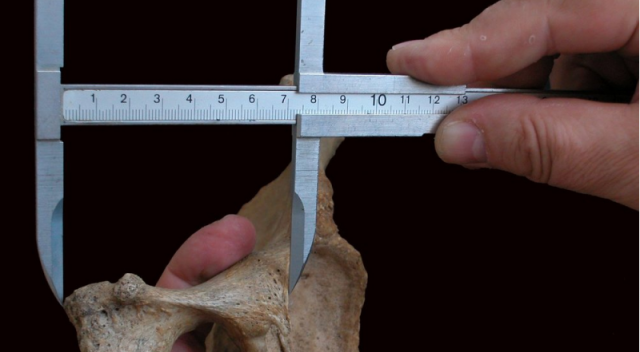
\includegraphics[width=0.5 \textwidth]{./pum.png}
\caption{Measurement PUM. \label{fig-pum}}
\end{figure}

\subsection{Statistical analysis}
\label{sec:org6d61bfe}
We performed a PCA using the R package \texttt{FactoMineR} \citep{le2008_FactoMineRPackageMultivariate}.

\section{Results}
\label{sec:org4aeaba0}
\subsection{Global morphology}
\label{sec:org0f3420c}
A PCA is shown on Figure \ref{fig-pca}.

\begin{figure}[htbp]
\centering
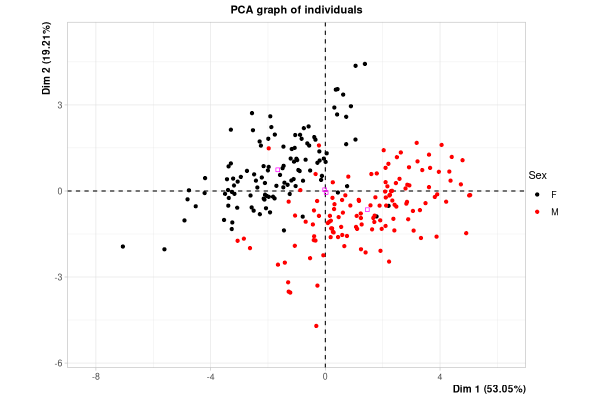
\includegraphics[width=.9\linewidth]{PCA.png}
\caption{A PCA on the reference sample. \label{fig-pca}}
\end{figure}

\subsection{Differences between the two collections}
\label{sec:orge8b2a2f}

\section{Discussion}
\label{sec:org2a9b1e2}
Aliquam erat volutpat.  Nunc eleifend leo vitae magna.  In id erat non orci commodo lobortis.  Proin neque massa, cursus ut, gravida ut, lobortis eget, lacus.  Sed diam.  Praesent fermentum tempor tellus.  Nullam tempus.  Mauris ac felis vel velit tristique imperdiet.  Donec at pede.  Etiam vel neque nec dui dignissim bibendum.  Vivamus id enim.  Phasellus neque orci, porta a, aliquet quis, semper a, massa.  Phasellus purus.  Pellentesque tristique imperdiet tortor.  Nam euismod tellus id erat.

\section{Conclusion}
\label{sec:org509faad}
Pellentesque dapibus suscipit ligula.  Donec posuere augue in quam.  Etiam vel tortor sodales tellus ultricies commodo.  Suspendisse potenti.  Aenean in sem ac leo mollis blandit.  Donec neque quam, dignissim in, mollis nec, sagittis eu, wisi.  Phasellus lacus.  Etiam laoreet quam sed arcu.  Phasellus at dui in ligula mollis ultricies.  Integer placerat tristique nisl.  Praesent augue.  Fusce commodo.  Vestibulum convallis, lorem a tempus semper, dui dui euismod elit, vitae placerat urna tortor vitae lacus.  Nullam libero mauris, consequat quis, varius et, dictum id, arcu.  Mauris mollis tincidunt felis.  Aliquam feugiat tellus ut neque.  Nulla facilisis, risus a rhoncus fermentum, tellus tellus lacinia purus, et dictum nunc justo sit amet elit.

\bibliography{../../../../complete_biblio}
\end{document}